\documentclass{beamer}
\beamertemplatenavigationsymbolsempty
\usecolortheme{beaver}
\setbeamertemplate{blocks}[rounded=true, shadow=true]
\setbeamertemplate{footline}[page number]
%
\usepackage[utf8]{inputenc}
\usepackage[english,russian]{babel}
\usepackage{amssymb,amsfonts,amsmath,mathtext}
\usepackage{subfig}
\usepackage[all]{xy} % xy package for diagrams
\usepackage{array}
\usepackage{multicol}% many columns in slide
\usepackage{hyperref}% urls
\usepackage{hhline}%tables
% Your figures are here:
\graphicspath{ {../figures/} }

%----------------------------------------------------------------------------------------------------------
\begin{document}
%----------------------------------------------------------------------------------------------------------
\begin{frame}[noframenumbering, plain]{Дистилляция в глубоких сетях и выравнивание структур}

    \begin{columns}[c]
        \column{0.4\textwidth}
        \begin{figure}
            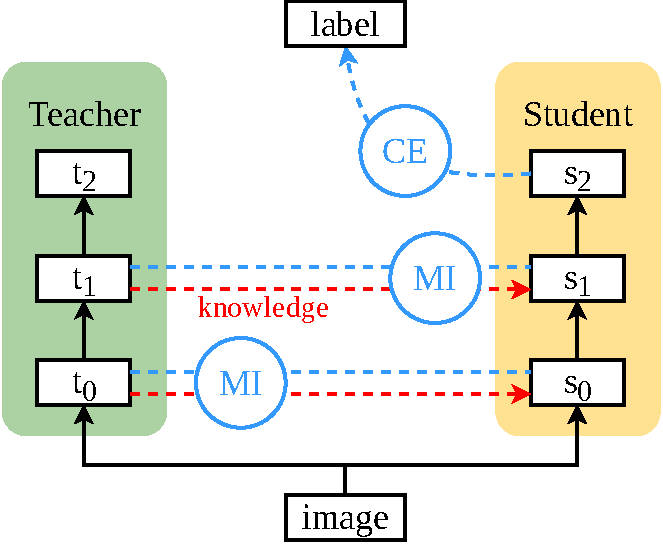
\includegraphics[width=1.0\textwidth]{ahn_diagram.pdf}
            \caption{Базовый метод}
        \end{figure}

        \column{0.4\textwidth}
        \begin{figure}
            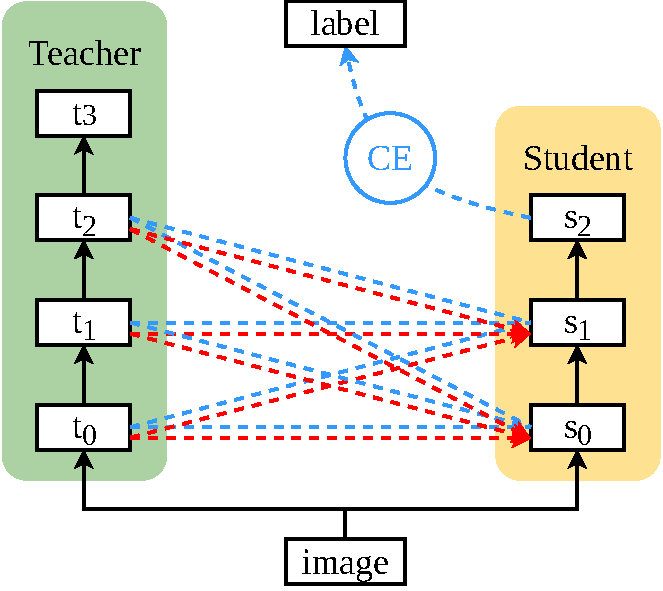
\includegraphics[width=1.0\textwidth]{our_diagram.pdf}
            \caption{Предлагаемый метод}
        \end{figure}
    \end{columns}

    \begin{columns}[c]
        \column{0.6\textwidth}
        \begin{equation}
            \mathcal{L} = \beta \mathcal{L}_\text{CE} + (1 - \beta){\sum_{i, j=1}^{T, S}\lambda_{i, j}I(t_{i}, s_{j})}
        \end{equation}
        \vspace*{-\baselineskip}\setlength\belowdisplayshortskip{0pt}
        \begin{equation}
            \forall i \hookrightarrow  \sum_{j=1}^{S}\lambda_{i, j} = 1
        \end{equation}

        \column{0.4\textwidth}
        $T, S$ - количество слоёв учителя и ученика,

        $I(t_{i}, s_{j})$ - взаимная информация,

        $\beta$ и $\lambda_{i, j}$ --- гиперпараметры.
    \end{columns}

\end{frame}
%----------------------------------------------------------------------------------------------------------

\end{document}